% Options for packages loaded elsewhere
\PassOptionsToPackage{unicode}{hyperref}
\PassOptionsToPackage{hyphens}{url}
%
\documentclass[
  ,jou,floatsintext]{apa6}
\usepackage{amsmath,amssymb}
\usepackage{lmodern}
\usepackage{iftex}
\ifPDFTeX
  \usepackage[T1]{fontenc}
  \usepackage[utf8]{inputenc}
  \usepackage{textcomp} % provide euro and other symbols
\else % if luatex or xetex
  \usepackage{unicode-math}
  \defaultfontfeatures{Scale=MatchLowercase}
  \defaultfontfeatures[\rmfamily]{Ligatures=TeX,Scale=1}
\fi
% Use upquote if available, for straight quotes in verbatim environments
\IfFileExists{upquote.sty}{\usepackage{upquote}}{}
\IfFileExists{microtype.sty}{% use microtype if available
  \usepackage[]{microtype}
  \UseMicrotypeSet[protrusion]{basicmath} % disable protrusion for tt fonts
}{}
\makeatletter
\@ifundefined{KOMAClassName}{% if non-KOMA class
  \IfFileExists{parskip.sty}{%
    \usepackage{parskip}
  }{% else
    \setlength{\parindent}{0pt}
    \setlength{\parskip}{6pt plus 2pt minus 1pt}}
}{% if KOMA class
  \KOMAoptions{parskip=half}}
\makeatother
\usepackage{xcolor}
\usepackage{graphicx}
\makeatletter
\def\maxwidth{\ifdim\Gin@nat@width>\linewidth\linewidth\else\Gin@nat@width\fi}
\def\maxheight{\ifdim\Gin@nat@height>\textheight\textheight\else\Gin@nat@height\fi}
\makeatother
% Scale images if necessary, so that they will not overflow the page
% margins by default, and it is still possible to overwrite the defaults
% using explicit options in \includegraphics[width, height, ...]{}
\setkeys{Gin}{width=\maxwidth,height=\maxheight,keepaspectratio}
% Set default figure placement to htbp
\makeatletter
\def\fps@figure{htbp}
\makeatother
\setlength{\emergencystretch}{3em} % prevent overfull lines
\providecommand{\tightlist}{%
  \setlength{\itemsep}{0pt}\setlength{\parskip}{0pt}}
\setcounter{secnumdepth}{-\maxdimen} % remove section numbering
% Make \paragraph and \subparagraph free-standing
\ifx\paragraph\undefined\else
  \let\oldparagraph\paragraph
  \renewcommand{\paragraph}[1]{\oldparagraph{#1}\mbox{}}
\fi
\ifx\subparagraph\undefined\else
  \let\oldsubparagraph\subparagraph
  \renewcommand{\subparagraph}[1]{\oldsubparagraph{#1}\mbox{}}
\fi
\newlength{\cslhangindent}
\setlength{\cslhangindent}{1.5em}
\newlength{\csllabelwidth}
\setlength{\csllabelwidth}{3em}
\newlength{\cslentryspacingunit} % times entry-spacing
\setlength{\cslentryspacingunit}{\parskip}
\newenvironment{CSLReferences}[2] % #1 hanging-ident, #2 entry spacing
 {% don't indent paragraphs
  \setlength{\parindent}{0pt}
  % turn on hanging indent if param 1 is 1
  \ifodd #1
  \let\oldpar\par
  \def\par{\hangindent=\cslhangindent\oldpar}
  \fi
  % set entry spacing
  \setlength{\parskip}{#2\cslentryspacingunit}
 }%
 {}
\usepackage{calc}
\newcommand{\CSLBlock}[1]{#1\hfill\break}
\newcommand{\CSLLeftMargin}[1]{\parbox[t]{\csllabelwidth}{#1}}
\newcommand{\CSLRightInline}[1]{\parbox[t]{\linewidth - \csllabelwidth}{#1}\break}
\newcommand{\CSLIndent}[1]{\hspace{\cslhangindent}#1}
\ifLuaTeX
\usepackage[bidi=basic]{babel}
\else
\usepackage[bidi=default]{babel}
\fi
\babelprovide[main,import]{english}
% get rid of language-specific shorthands (see #6817):
\let\LanguageShortHands\languageshorthands
\def\languageshorthands#1{}
% Manuscript styling
\usepackage{upgreek}
\captionsetup{font=singlespacing,justification=justified}

% Table formatting
\usepackage{longtable}
\usepackage{lscape}
% \usepackage[counterclockwise]{rotating}   % Landscape page setup for large tables
\usepackage{multirow}		% Table styling
\usepackage{tabularx}		% Control Column width
\usepackage[flushleft]{threeparttable}	% Allows for three part tables with a specified notes section
\usepackage{threeparttablex}            % Lets threeparttable work with longtable

% Create new environments so endfloat can handle them
% \newenvironment{ltable}
%   {\begin{landscape}\centering\begin{threeparttable}}
%   {\end{threeparttable}\end{landscape}}
\newenvironment{lltable}{\begin{landscape}\centering\begin{ThreePartTable}}{\end{ThreePartTable}\end{landscape}}

% Enables adjusting longtable caption width to table width
% Solution found at http://golatex.de/longtable-mit-caption-so-breit-wie-die-tabelle-t15767.html
\makeatletter
\newcommand\LastLTentrywidth{1em}
\newlength\longtablewidth
\setlength{\longtablewidth}{1in}
\newcommand{\getlongtablewidth}{\begingroup \ifcsname LT@\roman{LT@tables}\endcsname \global\longtablewidth=0pt \renewcommand{\LT@entry}[2]{\global\advance\longtablewidth by ##2\relax\gdef\LastLTentrywidth{##2}}\@nameuse{LT@\roman{LT@tables}} \fi \endgroup}

% \setlength{\parindent}{0.5in}
% \setlength{\parskip}{0pt plus 0pt minus 0pt}

% Overwrite redefinition of paragraph and subparagraph by the default LaTeX template
% See https://github.com/crsh/papaja/issues/292
\makeatletter
\renewcommand{\paragraph}{\@startsection{paragraph}{4}{\parindent}%
  {0\baselineskip \@plus 0.2ex \@minus 0.2ex}%
  {-1em}%
  {\normalfont\normalsize\bfseries\itshape\typesectitle}}

\renewcommand{\subparagraph}[1]{\@startsection{subparagraph}{5}{1em}%
  {0\baselineskip \@plus 0.2ex \@minus 0.2ex}%
  {-\z@\relax}%
  {\normalfont\normalsize\itshape\hspace{\parindent}{#1}\textit{\addperi}}{\relax}}
\makeatother

% \usepackage{etoolbox}
\makeatletter
\patchcmd{\HyOrg@maketitle}
  {\section{\normalfont\normalsize\abstractname}}
  {\section*{\normalfont\normalsize\abstractname}}
  {}{\typeout{Failed to patch abstract.}}
\patchcmd{\HyOrg@maketitle}
  {\section{\protect\normalfont{\@title}}}
  {\section*{\protect\normalfont{\@title}}}
  {}{\typeout{Failed to patch title.}}
\makeatother

\usepackage{xpatch}
\makeatletter
\xapptocmd\appendix
  {\xapptocmd\section
    {\addcontentsline{toc}{section}{\appendixname\ifoneappendix\else~\theappendix\fi\\: #1}}
    {}{\InnerPatchFailed}%
  }
{}{\PatchFailed}
\usepackage{dblfloatfix}


\usepackage{csquotes}
\ifLuaTeX
  \usepackage{selnolig}  % disable illegal ligatures
\fi
\IfFileExists{bookmark.sty}{\usepackage{bookmark}}{\usepackage{hyperref}}
\IfFileExists{xurl.sty}{\usepackage{xurl}}{} % add URL line breaks if available
\urlstyle{same} % disable monospaced font for URLs
\hypersetup{
  pdftitle={Faith in Reason: developing a survey measure of belief in the rationality of others},
  pdfauthor={Tom Stafford1, Junyan Zhu2, \& Katharine Dommett2},
  pdflang={en-EN},
  hidelinks,
  pdfcreator={LaTeX via pandoc}}

\title{Faith in Reason: developing a survey measure of belief in the rationality of others}
\author{Tom Stafford\textsuperscript{1}, Junyan Zhu\textsuperscript{2}, \& Katharine Dommett\textsuperscript{2}}
\date{}


\shorttitle{Faith in Reason}

\authornote{

For the purpose of open access, the author has applied a Creative Commons Attribution (CC BY) licence to any Author Accepted Manuscript version arising.

Document prepared with RMarkdown (Allaire et al., 2020) and papaja (Aust \& Barth, 2020). CRediT (Contributor Roles Taxonomy) autogenerated using Tenzing (Holcombe, Kovacs, Aust, \& Aczel, 2020). Template is available here \href{https://github.com/tomstafford/rmarkdown_apa}{github.com/tomstafford/rmarkdown\_apa}

The authors made the following contributions. Tom Stafford: Conceptualization, Data curation, Formal analysis, Funding acquisition, Methodology, Visualization, Writing - original draft, Writing - review \& editing; Junyan Zhu: Conceptualization, Data curation, Formal analysis, Methodology, Visualization, Writing - original draft, Writing - review \& editing; Katharine Dommett: Conceptualization, Funding acquisition, Methodology, Writing - review \& editing.

Correspondence concerning this article should be addressed to Tom Stafford, Department of Psychology, University of Sheffield, Sheffield, UK. E-mail: \href{mailto:t.stafford@sheffield.ac.uk}{\nolinkurl{t.stafford@sheffield.ac.uk}}

}

\affiliation{\vspace{0.5cm}\textsuperscript{1} Department of Psychology, University of Sheffield, UK\\\textsuperscript{2} Department of Politics and International Relations, University of Sheffield, UK}

\note{\textcolor{red}{Preprint 2023-04-01}}

\abstract{%
abstract goes here
}



\begin{document}
\maketitle

\hypertarget{introduction}{%
\section{Introduction}\label{introduction}}

What we believe about other people matters. It is not enough that others are trustworthy, reasonable or well intentioned. Successful coordination, as well as individual wellbeing, benefit when we also \emph{perceive} others as trustworthy, reasonable or well intentioned.

\hypertarget{generalised-trust}{%
\subsection{Generalised trust}\label{generalised-trust}}

\hypertarget{second-order-effexcts-of-disinfo}{%
\subsection{Second order effexcts of Disinfo}\label{second-order-effexcts-of-disinfo}}

Karpf D (2019) On digital disinformation and democratic myths. Mediawell. Available at: \url{https://mediawell.ssrc.org/expert-reflections/on-digital-disinformation-and-democratic-myths/}

Hoes E, Clemm B, Gessler T, et al.~(2022) The Cure Worse Than the Disease? PsyArXiv. Available at: \url{https://doi.org/10.31234/osf.io/4m92p}

Jungherr A, Rauchfleisch A (2022) Negative downstream effects of disinformation discourse: evidence from the US. SocArXiv.

Lee T (2021) How people perceive influence of fake news and why it matters. Communication Quarterly 69(4): 431--453.

Nisbet EC, Mortenson C, Li Q (2021) The presumed influence of election misinformation on others reduces our own satisfaction with democracy. The Harvard Kennedy School (HKS) Misinformation Review. Available at: \url{https://misinforeview.hks.harvard.edu/article/the-presumed-influence-of-election-misinformation-on-others-reduces-our-own-satisfaction-with-democracy/}

Nyhan B (2020) Facts and myths about misperceptions. Journal of Economic Perspectives 34(3): 220--236.

\hypertarget{third-person-effect}{%
\subsection{Third person effect}\label{third-person-effect}}

\begin{itemize}
\item
  Some part of the TPE may be driven by accurate perception of others
  Lyons B (2022) Why we should rethink the third-person effect: Disentangling bias and earned confidence. Available at: \url{https://www.dropbox.com/s/tpzy6e1ovfi0y1o/Why\%20we\%20should\%20rethink\%20TPE\%20\%28v2\%2C\%202022\%29.pdf?dl=0}
\item
  driving calls for censorship
  Olshansky A, Landrum AR (2020) Third-person perceptions and calls for censorship of Flat Earth videos on YouTube. Media and Communication 8(2): 387--400.
  Feng GC, Guo SZ (2012) Support for censorship: a multilevel meta-analysis of the third-person effect. Communication Reports 25(1): 40--50.
\end{itemize}

\hypertarget{rationality}{%
\subsection{Rationality}\label{rationality}}

Dawson, N. V., \& Gregory, F. (2009). Correspondence and coherence in science: A brief historical perspective. Judgment and decision making, 4(2), 126-133.

\hypertarget{insight}{%
\subsubsection{Insight}\label{insight}}

Nisbett, R. E., \& Wilson, T. D. (1977). Telling more than we can know: Verbal reports on mental processes. Psychological review, 84(3), 231.

\hypertarget{influence-gullibility}{%
\subsubsection{Influence / Gullibility}\label{influence-gullibility}}

Altay, S., \& Acerbi, A. (2023). People believe misinformation is a threat because they assume others are gullible. New Media \& Society, 0(0). \url{https://doi.org/10.1177/14614448231153379}

Confidence in their abilities, friends' and family's abilities, and people's abilities to spot misinformation was measured with three statements adapted from Corbu et al.~(2020) and the European Commission (2018):
``I am able to identify news or information that misrepresent reality or is even false''
``My friends and family are able to identify news or information that misrepresent reality or is even false''
``People in general are able to identify news or information that misrepresent reality or is even false''

\begin{itemize}
\tightlist
\item
  negatively conceived
\item
  unidimensional: influence
\end{itemize}

\hypertarget{method}{%
\section{Method}\label{method}}

Part of a larger survey

\hypertarget{sample}{%
\subsection{Sample}\label{sample}}

\hypertarget{item-development}{%
\subsection{Item development}\label{item-development}}

correspondance (items 2 and 6)
coherance (items 7 and 8)
influence (items 3 and 5)
insight into behaviour (4)
naive endorsement (item 1)

See Table \ref{tab:items}

\begin{table*}[tbp]

\begin{center}
\begin{threeparttable}

\caption{\label{tab:items}Scale item wording}

\begin{tabular}{ll}
\toprule
nums & \multicolumn{1}{c}{items}\\
\midrule
1 & The typical person is often irrational\\
2 & People are often misinformed on important issues\\
3 & People are too easily manipulated\\
4 & People often act for reasons they don’t understand or endorse\\
5 & The average person can be persuaded to change their mind if given good reasons\\
6 & Most people hold accurate views about the world\\
A & For this question please click the middle option, ‘neutral’, to show you are paying attention\\
7 & An individual's beliefs about the world are generally coherent\\
8 & People's behaviour is generally consistent with their beliefs\\
\bottomrule
\addlinespace
\end{tabular}

\begin{tablenotes}[para]
\normalsize{\textit{Note.} Response was on a 7 point Likert scale from (1 = "Strong Disagree", 7 = "Strongly Agree"). Items 1,2,3 and 4 reverse coded so that for all items higher scores represented stronger faith in reason.}
\end{tablenotes}

\end{threeparttable}
\end{center}

\end{table*}

\hypertarget{prereg}{%
\subsection{Prereg}\label{prereg}}

\hypertarget{reproducibility}{%
\subsection{Reproducibility}\label{reproducibility}}

Code and data is open

Reproducible manuscript, origin files at \url{https://github.com/tomstafford/faithinreason}

\hypertarget{results}{%
\section{Results}\label{results}}

Our data consist of 1875 participants who completed our online survey. 6 failed an attention check and were removed.

\begin{figure}

{\centering 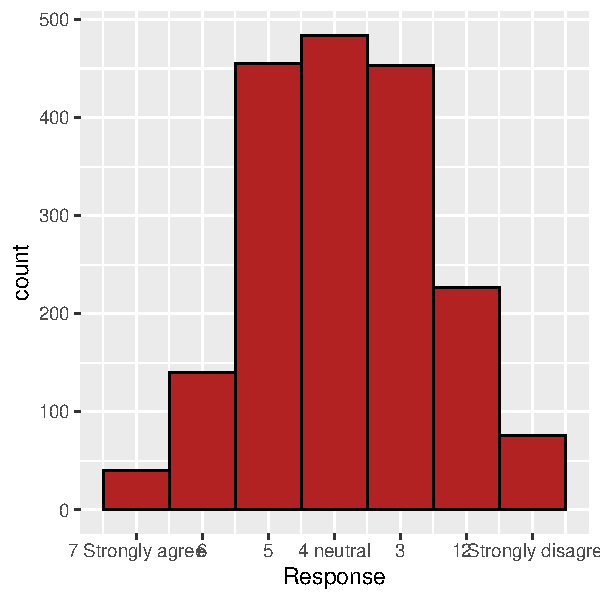
\includegraphics[width=0.75\linewidth]{faithinreason_files/figure-latex/ourhistogram-1} 

}

\caption{Histogram of responses to Item 1 ("The typical person is often irrational")}\label{fig:ourhistogram}
\end{figure}

We asked 8 questions about rationality in the survey. To determine the homogeneity and the
fitness of the responses, I use Stata to perform Mokken scaling analysis. Testing all 8
rationality variables, the Mokken analysis yields one scale of 6 items. The items with low
Loevinger's coefficient of homogeneity (H i ), a criterion for scalability, are dropped. If the
overall H\textless0.3, it means the items in the scale are unrelated, thus cannot be accepted to form a
cumulative scale. As a rule of thumb, H i must be higher than 0.3 to be kept in the scale.
Therefore, there are 6 fitting items in the scale: rationality\_1, rationality\_2, rationality\_3,
rationality\_4, rationality\_6, and rationality\_7. The overall H coefficient is 0.41, indicating a
medium-strong scalability. The individual critical values in the scale are all lower than 80, so
the variables are double monotonous and there is no model violation.
Code: loevh rationality\_1 rationality\_2 rationality\_3 rationality\_4 rationality\_6 rationality\_7,
pair monotonicity(*) ppp pmm nipmatrix(minvi(0.03) siglevel(0.01))
We can thus generate a rationality variable by aggregating those six variables. Cronbach's \(\alpha\)
is 0.78, indicating an acceptable internal consistency.

Based on the statistical results, it looks to me that rationality\_5 (The average person can be
persuaded to change if given good reasons) is a real problem, it doesn't fit at all with other items

3
and must be removed. Rationality\_8 (People\textquotesingle s behaviour is generally consistent with their beliefs)
has a poor fitness, but it is not as bad as rationality\_5.

Next, I try to scale the remaining two items that are not included in the above scale --
rationality\_5 and rationality\_8. As expected, these two items doesn't form a separate scale.
Empirically, these items are excluded from the rationality measure by Mokken scaling likely
because persuasion effect is not a robust indication of rationality?

\hypertarget{discussion}{%
\section{Discussion}\label{discussion}}

\hypertarget{normative-models}{%
\subsection{Normative models}\label{normative-models}}

arguably our scale doesn't touch on normative models of rationality as captured by T\&K. Bias, prejudice

\hypertarget{references}{%
\section*{References}\label{references}}
\addcontentsline{toc}{section}{References}

\hypertarget{refs}{}
\begin{CSLReferences}{1}{0}
\leavevmode\vadjust pre{\hypertarget{ref-rmarkdowncite}{}}%
Allaire, J., Xie, Y., McPherson, J., Luraschi, J., Ushey, K., Atkins, A., \ldots{} Iannone, R. (2020). \emph{Rmarkdown: Dynamic documents for r}. Retrieved from \url{https://github.com/rstudio/rmarkdown}

\leavevmode\vadjust pre{\hypertarget{ref-aust2020}{}}%
Aust, F., \& Barth, M. (2020). \emph{{papaja}: {Create} {APA} manuscripts with {R Markdown}}. Retrieved from \url{https://github.com/crsh/papaja}

\leavevmode\vadjust pre{\hypertarget{ref-holcombe2020documenting}{}}%
Holcombe, A. O., Kovacs, M., Aust, F., \& Aczel, B. (2020). Documenting contributions to scholarly articles using CRediT and tenzing. \emph{PLoS One}, \emph{15}(12), e0244611.

\end{CSLReferences}


\end{document}
